\subsubsection{Firmware Elements}

The firmware elements, shown in Fig.~\ref{fig:block-software}, are detailedbelow. The detailed implementation of these elements is given in \cite{flightcontroller_git}. To view the code as up to date with the submission of this report, refer to Appendix~\ref{app:firmware-code}.

\begin{figure}[H]
    \centering
    \captionsetup{justification=centering, margin=1cm}
    
\includegraphics[width=0.45\textwidth]{img/firmware-flavour2.jpeg}
    \caption{\gls{esp-idf} Environment}
    \label{fig:frame}
\end{figure}

\paragraph{\textbf{Sensor Task} \textit{sensors.c}} \leavevmode

The sensor task provides an interface for the \gls{mpu6050} 6-axis \gls{imu} through \gls{i2c}, which provides real-time data from the accelerometer and gyroscope on the sensor. This is done on a register level using Espressif's \textit{I2C} library.

An \gls{isr} is attached to the \gls{mpu6050} interrupt; this means that instead of the sensor task continuously reading from the \gls{mpu6050}, it waits for the trigger to signify that data is ready to be read. The data is then stored in a queue, and an additional signal is sent to the stabiliser task to signify the processed sensor data is ready.

\begin{figure}[H]
    \centering
    \captionsetup{justification=centering, margin=1cm}
    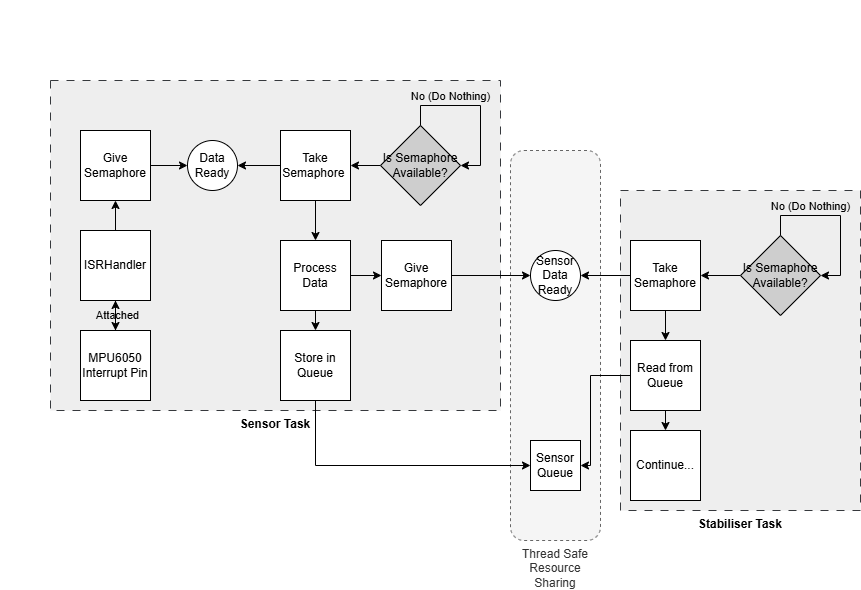
\includegraphics[width=0.85\textwidth]{img/sensor-semaphore.PNG}
    \caption{Thread-safe Data Availability Signalling Heuristic}
    \label{fig:isr}
\end{figure}

The raw data obtained from the \gls{mpu6050} sensor are 16-bit integer values representing the gyroscope and accelerometer measurements. These values are first converted into physical units (SI units) based on the selected sensitivity configuration of the sensor. The conversion from raw readings to angular velocity and linear acceleration is expressed as:

\begin{align}
\boldsymbol{\omega} &= (\mathbf{G}_{\text{raw}} - \mathbf{G}_{\text{bias}}) \times S_{\text{gyro}}, \\[6pt]
\mathbf{a} &= \mathbf{A}_{\text{raw}} \times S_{\text{acc}},
\end{align}

where \( \mathbf{G}_{\text{raw}} \) and \( \mathbf{A}_{\text{raw}} \) are the raw gyroscope and accelerometer readings, \( \mathbf{G}_{\text{bias}} \) is the gyroscope bias, which is calculated when the filter is initialised. \( S_{\text{gyro}} \) and \( S_{\text{acc}} \) are the corresponding sensitivity scaling factors.

To reduce measurement noise, a second-order digital biquad low-pass filter is applied to the sensor data. This filter attenuates high-frequency noise while preserving the motion dynamics of interest. Cutoff frequencies of 30\,Hz and 80\,Hz are used for the accelerometer and gyroscope, respectively. Additionally, the \gls{mpu6050} incorporates an internal digital low-pass filter on the gyroscope measurements, which is also enabled for further signal smoothing. The digital biquad filter can be expressed in the $z$-domain as:

\begin{align}
H(z) &= \frac{b_0 + b_1 z^{-1} + b_2 z^{-2}}{1 + a_1 z^{-1} + a_2 z^{-2}}, \\[6pt]
w(n) &= x(n) - a_1 w(n-1) - a_2 w(n-2), \\[6pt]
y(n) &= b_0 w(n) + b_1 w(n-1) + b_2 w(n-2),
\end{align}

where \( x(n) \) is the current input sample, \( y(n) \) is the filtered output, and \( w(n) \) represents the internal state variables in Direct Form~II. The coefficients can be found in~\ref{app:code-filter}.

\paragraph{\textbf{State Estimation} \textit{estimator.c}} \leavevmode 

The \gls{mpu6050} measures angular rate from the gyroscope and linear acceleration from the accelerometer, which do not directly provide information about its orientation or position in space. The drone does not have inherent knowledge of its position relative to world coordinates. Simple integration can be used to estimate this, but leads to errors also accumulating.

\begin{figure}[H]
    \centering
    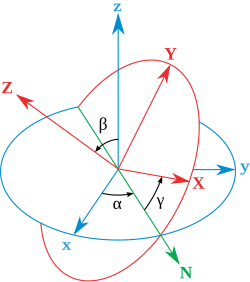
\includegraphics[width=0.25\textwidth]{img/euler.PNG}
    \caption{Euler Angles~\cite{euler_angles_wikipedia}}
\end{figure}

The quaternion number system extends complex numbers to three dimensions. The detailed mathematics are omitted here, but practically it solves issues with the Euler angle system. One issue with this system is gimbal lock: when two of the three Euler axes align, a degree of freedom is lost. This does not mean the axes are physically locked but causes unpredictable movement.

Quaternions and an \gls{ahrs} algorithm called Mahony's algorithm are used in the CrazyFlie firmware to achieve state estimation, which has been adapted for the firmware in this project. This estimate is sent to the WebSocket for visualisation.

\begin{figure}[H]
    \centering
    \captionsetup{justification=centering, margin=1cm}
    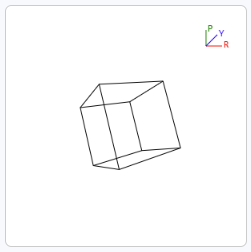
\includegraphics[width=0.4\textwidth]{img/websocket-state.PNG}
    \caption{Real-Time State Estimate Display on WebSocket}
    \label{fig:ws-state}
\end{figure}

\paragraph{\textbf{Controller} \textit{controller.c}} \leavevmode 

Once the state estimate is received and the setpoint is received, representing the current and desired states, the realisation of the control to reach the setpoint is met through the use of a control system, in this case a cascaded \gls{pid} loop. The system consists of two nested loops:

\begin{itemize}
    \item \textbf{Outer Loop (Attitude Control):} Computes desired angular rates from the error between the target attitude (roll, pitch, yaw) and the current attitude measured by the \gls{imu}. Separate \gls{pid} objects are used for each axis.
    \item \textbf{Inner Loop (Rate Control):} Converts the desired angular rates into motor commands. This loop uses the gyroscope measurements to reduce the angular rate error and generate the control outputs sent to the motors.
\end{itemize}

For each control cycle, the process is:

\begin{enumerate}
    \item Update the desired attitude based on setpoints or manual input.
    \item Compute the attitude error and update the attitude \gls{pid} to get desired angular rates.
    \item Update the angular rate \gls{pid} using gyroscope measurements to produce motor outputs.
    \item Saturate and scale outputs to safe ranges for \gls{pwm} signals.
\end{enumerate}

This cascaded \gls{pid} structure allows stable hovering and responsive attitude control while decoupling the slower attitude loop from the faster rate loop, providing robust control.

\pagebreak
\paragraph{\textbf{Stabiliser} \textit{stabiliser.c}} \leavevmode

The stabiliser ensures that all other processes in the flight controller run on time and repeatedly, acting as the centralised task from which other functions are called. A key feature is its timing system: different parts of the controller run at different frequencies using a tick-based approach. This applies both in the state estimator, which updates the attitude and position estimates, and in the controller, which computes the control outputs.  

\begin{figure}[H]
    \centering
    \captionsetup{justification=centering, margin=1cm}
    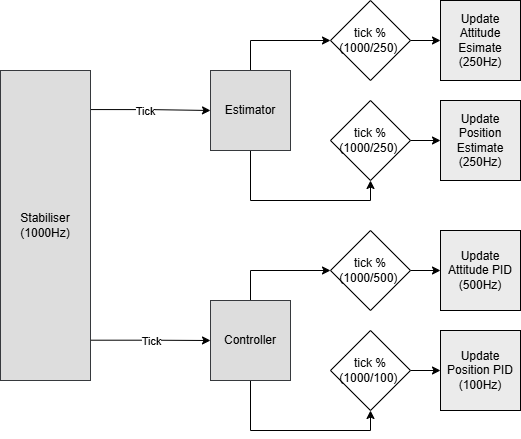
\includegraphics[width=0.53\textwidth]{img/timing.PNG}
    \caption{Simplified Timing Description}
\end{figure}

For stabilisation, the attitude loop, controlling roll, pitch, and yaw, runs at a high frequency (500~Hz) to respond quickly to rapid angular changes. The position loop, controlling altitude and horizontal position, runs at a lower frequency (100~Hz) since translational motion is slower. This setup ensures fast dynamics are stabilised quickly, while slower dynamics are controlled efficiently.

\paragraph{\textbf{WebSocket} \textit{websocket.c}} \leavevmode

The WebSocket interface provides a real-time connection between the flight controller and a web-based user interface. It allows the drone to send sensor readings, state estimates, and control outputs to the browser, while receiving setpoints and manual control commands from the user.  

The \gls{html} interface displays \gls{imu} data, attitude, position, and motor outputs, and provides sliders and buttons for manual control. The WebSocket ensures that these updates are transmitted asynchronously, so the stabiliser and controller loops continue running at their required rates. Users can enable or disable motors, adjust setpoints, and request telemetry in real time, with the interface handling both periodic state updates and on-demand commands efficiently. The WebSocket interface is given in Appendix~\ref{app:websocket}.

\paragraph{\textbf{Motors} \textit{motors.c}} \leavevmode

The motors module converts the outputs of the stabiliser and controller into signals for the four drone motors. The controller outputs \textit{thrust} and attitude control corrections (\textit{roll, pitch, yaw}) which are distributed to each motor to achieve the desired motion. 

\pagebreak
For a quadcopter in an X-configuration, the motor commands are calculated as:

\[
\begin{aligned}
M_1 &= T - \frac{R}{2} + \frac{P}{2} + Y \\
M_2 &= T - \frac{R}{2} - \frac{P}{2} - Y \\
M_3 &= T + \frac{R}{2} - \frac{P}{2} + Y \\
M_4 &= T + \frac{R}{2} + \frac{P}{2} - Y
\end{aligned}
\]

where \(M_i\) is the command for motor \(i\), \(T\) is the total thrust, \(R, P, Y\) are the roll, pitch, and yaw corrections respectively. The roll and pitch contributions are halved to balance their effect across opposing motors.  

Each motor command is then limited to a minimum \textit{idle thrust} to ensure stable spinning even when the drone is hovering:

\[
M_i = \max(M_i, T_\text{idle})
\]

Finally, these commands are converted to \gls{pwm} signals for the motor drivers with a linear mapping from the 16-bit thrust command to the duty cycle of the \gls{pwm} hardware:

\[
\text{PWM}_{i} = \text{motorConv16ToBits}(M_i)
\]

This mapping allows the controller outputs to directly control motor speeds, which in turn generate the required forces and torques to stabilise and manoeuvre the drone.